\documentclass[12pt, letterpaper]{article}
\usepackage[utf8]{inputenc}
\usepackage{amsmath}
\usepackage{changepage}% http://ctan.org/pkg/changepage
\usepackage{titlesec} 
\usepackage{placeins}
\usepackage{caption}
\newcommand\tab[1][1cm]{\hspace*{#1}}
\titleformat{\subsection}[runin]{}{}{}{}[]
\usepackage{graphicx}


\title{CS M148 Homework 2}
\author{Hanna Co}
\date{Due: February 16, 2021}

\begin{document}
\maketitle
\newpage
\section{Bias, Variance and Regularization}
\subsection*{a)} The graph on the far left has the largest bias and the lowest variance, and the graph on the far right has the largest variance and the lowest bias.
\begin{figure}[h!]
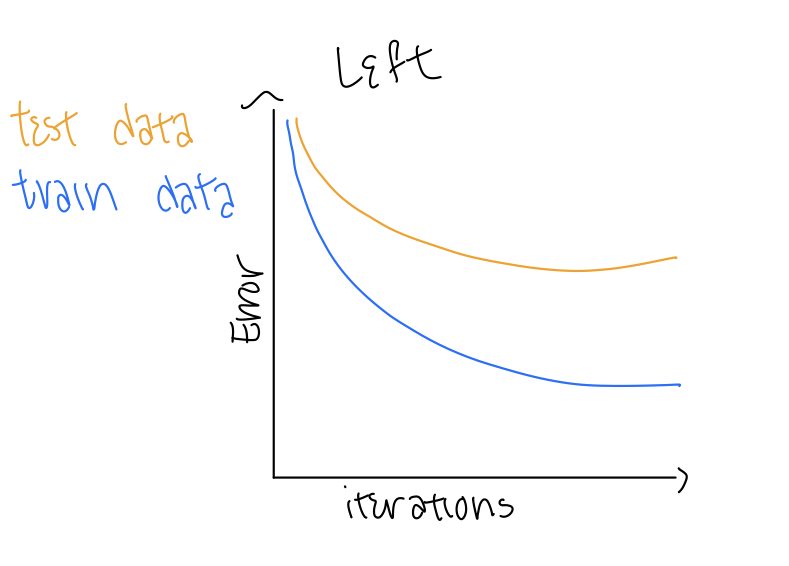
\includegraphics[scale=0.33]{./images/1a_left.jpg}
\caption*{The graph on the left will perform bad on both the train and test data, because it's too generalized.}
\end{figure}
\begin{figure}[h!]
  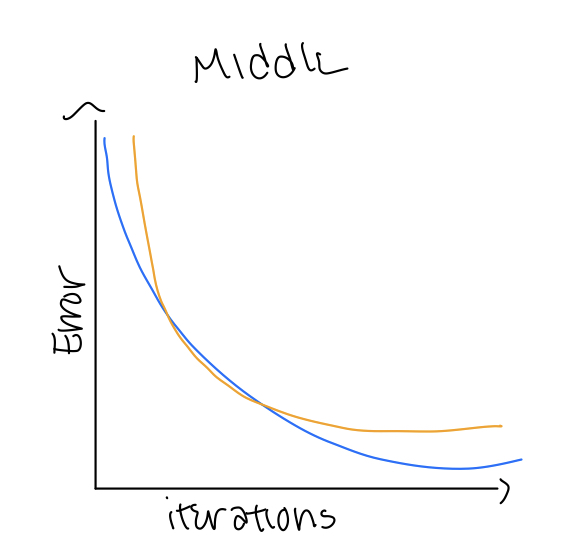
\includegraphics[scale=0.33]{./images/1a_middle.jpg}
\caption*{The graph in the middle will perfrom alright on both train and test data. This is because it's well fitted to the training data, but not overfitted to the point that it performs badly on test data.}
\end{figure}
\begin{figure}[h!]
  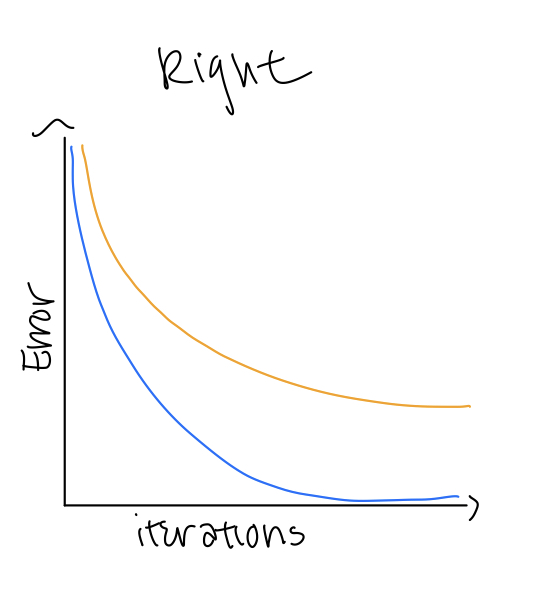
\includegraphics[scale=0.33]{./images/1a_right.jpg}
\caption*{The graph on the right will perform really good on the training data, but this is because it is overfitted to the training data. Thus, it will not perform will on the test data.}
\end{figure}
\clearpage

\subsection*{b)} L1 regularization is used on a), because the coefficients are nullified fast, compared to b), where they are not nullified.

\newpage
\section{Maximum Likelihood View of Linear Regression}
\subsection*{a)} Since the likelihood function represents the probability of producing a particular sample, thus the equation is:\\
$\prod_{i=1}^{n}\frac{1}{\sigma\sqrt{2\pi}}exp(\frac{-1}{2}(\frac{y_i-\hat{y_i}}{\sigma})^2)$\\

\subsection*{b)} We take the equation in 2a and change it into the log likelihood equation:\\
$\sum_{i=1}^{n}ln(\frac{1}{\sqrt{2\pi\sigma^2}}exp(-\frac{(y_i - \hat{y_i})^2}{2\sigma^2}))$\\
$\sum_{i=1}^{n}ln(\frac{1}{\sqrt{2\pi\sigma^2}}) -\frac{(y_i - \hat{y_i})^2}{2\sigma^2}$\\
$\sum_{i=1}^{n}-\frac{1}{2}ln(2\pi\sigma^2) -\frac{(y_i - \hat{y_i})^2}{2\sigma^2}$\\
$-\frac{n}{2}ln(2\pi\sigma^2) -\sum_{i=1}^{n}\frac{(y_i - \hat{y_i})^2}{2\sigma^2}$\\

We want to find $argmax(L)$:\\
$argmax(L) = argmax(-\sum_{i=1}^{n}\frac{(y_i - \hat{y_i})^2}{2\sigma^2})$\\
Since we will end up setting $argmax(L) = 0$, we can simply write\\
$argmax(L) = argmax(-\sum_{i=1}^{n}(y_i - \hat{y_i})^2)$\\
Since $argmax(L) = argmin(-L)$, \\
$argmax(L) = argmin(\sum_{i=1}^{n}(y_i - \hat{y_i})^2)$\\
Additionally, $n$ is a constant, so we have\\
$argmax(L) = argmin(\frac{1}{n}\sum_{i=1}^{n}(y_i - \hat{y_i})^2)$\\
$\hat{y_i}$ is our model, so we substitute $\hat{y_i}$ with $\beta_0 + \beta_1x_i$\\
$argmax(L) = argmin(\frac{1}{n}\sum_{i=1}^{n}(y_i - \beta_0 - \beta_1x_i)^2)$\\
Notice that the right hand side of the above equation is the equation for MSE. Thus, maximizing log likelihood is equivalent to maximizing MSE.

\newpage
\section{Classification Metric}
\subsection*{a)}ROC Curve
\FloatBarrier
\begin{figure}[h!]
  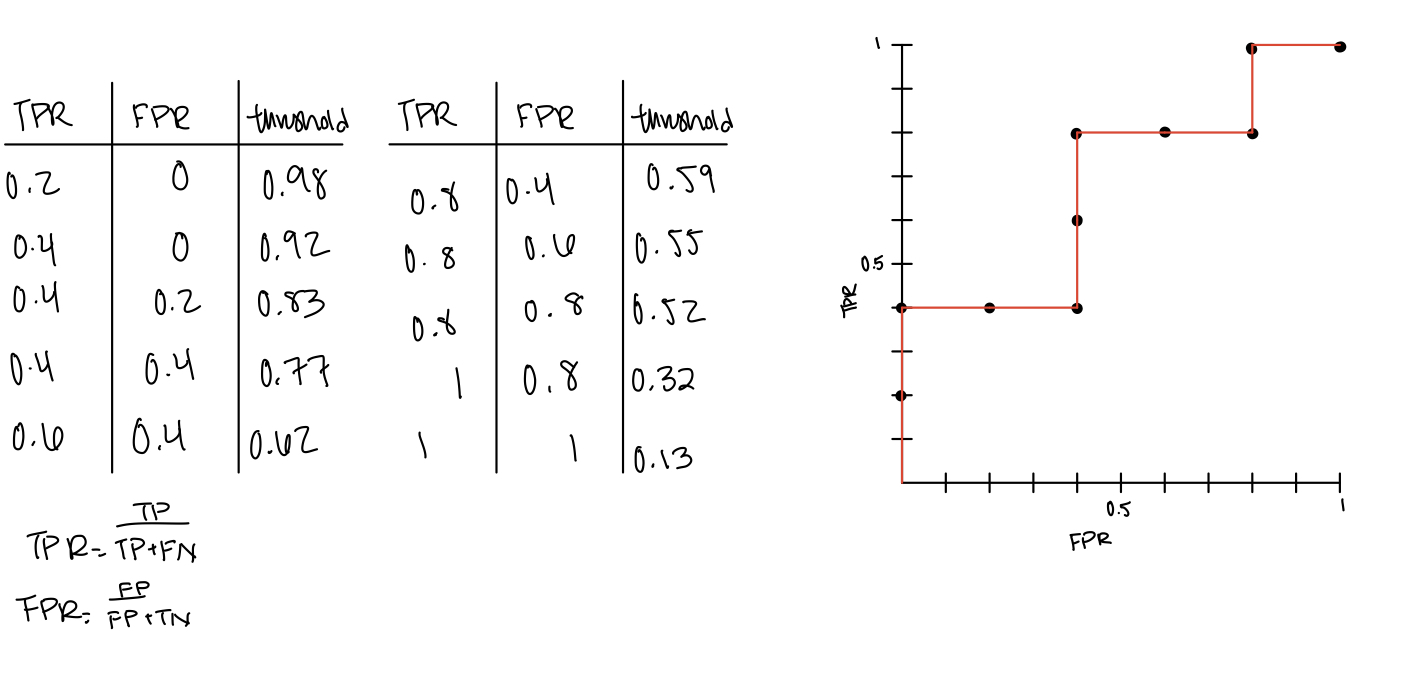
\includegraphics[scale=0.33]{./images/3a.jpg}
\end{figure}
\clearpage

\subsection*{b)} $(0.4)(1) + (0.4)(0.6) + (0.2)(0.2) = 0.68$

\subsection*{c)} Confusion Matrix
\FloatBarrier
\begin{figure}[h!]
  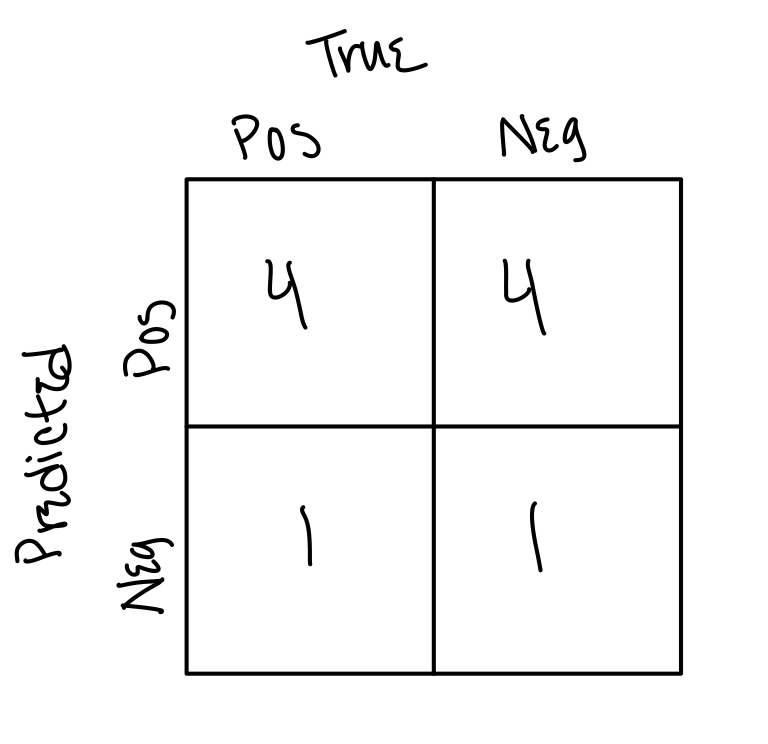
\includegraphics[scale=0.33]{./images/3c.jpg}
\end{figure}

\subsection*{d)} Accuracy = $\frac{TP + TN}{TP+FP+TN+FN} = \frac{4+1}{4+1+4+1} = 0.5$\\
Precision = $\frac{TP}{TP+FP} = \frac{4}{4+1} = 0.5$\\
Recall = $\frac{TP}{TP+FN} = \frac{4}{4+1} = 0.8$\\
F1 Score = $2 * \frac{precision * recall}{precision+recall} = 2*\frac{0.8*0.5}{0.8+0.5} = 0.615$

\subsection*{e)} Yes, we can improve the scores by changing our threshold to any value above 0.55, and less than or equal to 0.59.  This changes two of our false positives to true negatives. Our new accuracy is 0.7, our new precision is 0.67, our new f1 score is 0.73, and our recall remains at 0.8.

\newpage
\section{4 K-Nearest Neighbors for Classification}
\begin{figure}[h!]
  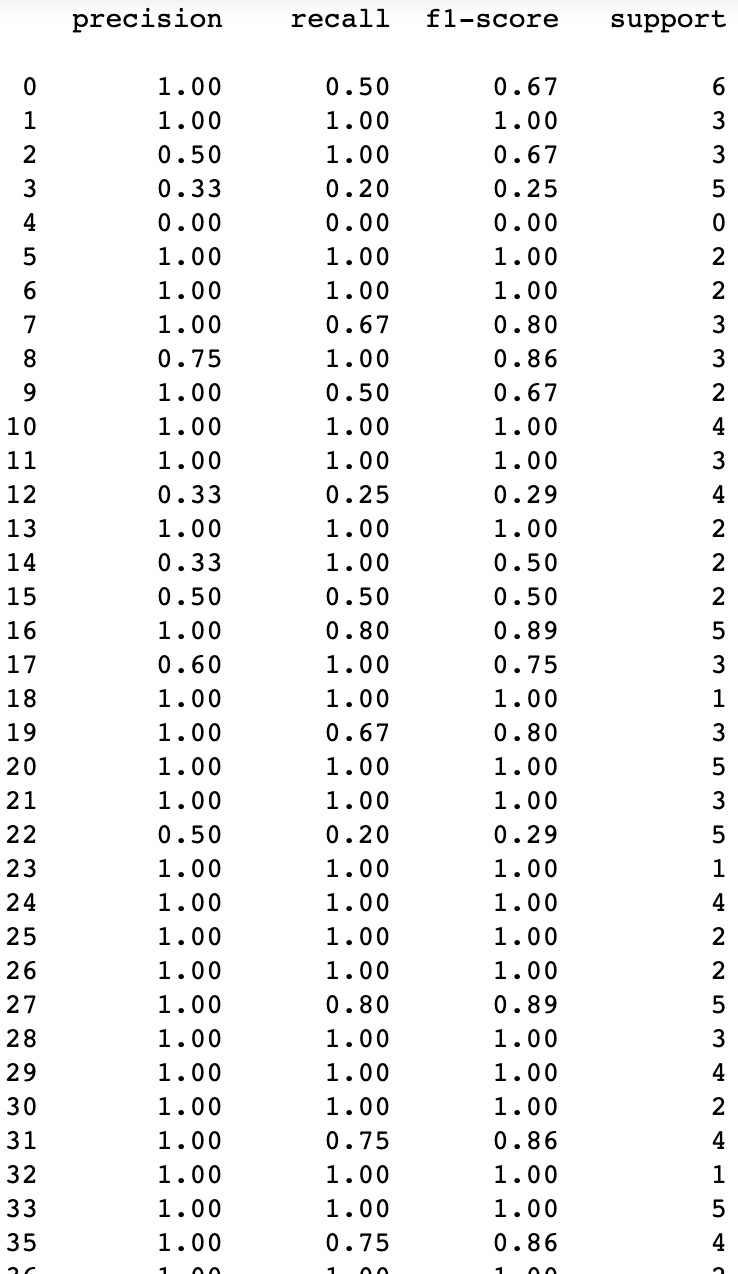
\includegraphics[scale=0.33]{./images/4.jpg}
\end{figure}
\subsection*{a)} The numbers are classes, and the lines include the precision, recall, f1 score and support for each class.

\subsection*{b)} For the most part, yes, though there are a few classes where it doesn't perform well. For example, class=12 and class=39 do not perform well in terms of the reported metrics.

\subsection*{c)} Yes, the results would be different if the lighting or angles of the faces varied more. This gives the model more variety to train on. The results could change with a different background -- if the contrast was similar to the current background, the results would probably be very similar. However, if it was changed to a low contrast background, it would likely make the model worse, because it becomes harder to differentiate between the face and the background.

\newpage
\section{Logistic Regression}
\subsection*{a)} We have the equation $ln(\frac{P(Y=1)}{1-P(Y=1)}) = \beta_0 + \beta_1X_1 + ... + \beta_pX_p$.\\
Since $X_1 = X_2 = 0,$ this equation becomes $ln(\frac{P(Y=1)}{1-P(Y=1)}) = \beta_0$.\\
$ln(\frac{P(Y=1)}{1-P(Y=1)}) = 3$.\\
$\frac{P(Y=1)}{1-P(Y=1)} = e^3$\\
$P(Y=1) = (1-P(Y=1))e^3$\\
$P(Y=1) = e^3-e^3P(Y=1)$\\
$P(Y=1) + e^3P(Y=1) = e^3$\\
$P(Y=1)*(1 + e^3) = e^3$\\
$P(Y=1) = \frac{e^3}{1 + e^3}$\\
$P(Y=1) = 0.953$\\
$\frac{P(Y=1)}{1-P(Y=1)} = 20.086$\\
The probability of the event Y=1 is 0.953, and the odds are 20.086.\\
\subsection*{b)} A one unit increase in $X_1$ increases our log odds by 2 and our odds by a factor of $e^2$. A one unit increase in $X_2$ decreases our log odds by 5 and our odds by a factor of $e^{-5}$.

\subsection*{c)} Increasing $\beta_0, \beta_1, \beta_2$ will increase both our odds and log odds, while decreasing them would decrease our odds and log odds. Increasing $\beta_0$ by one will increase our log odds by 1 and our odds by a factor of $e^1$, and decreasing $\beta_0$ will decrease our log odds by 1 and our odds by a factor of $e^1$. As for $\beta_1$ and $\beta_2$, assuming that $X_1$ and $X_2$ are kept the same, then increasing $\beta_1$ by one will increase our log odds by $X_1$, and our odds by $e^{X_1}$ and decreasing $\beta_1$ by one will decrease our log odds by $X_1$. and our odds by $e^{X_1}$ Similarly, increasing $\beta_2$ by one will increase our log odds by $X_2$ and our odds by a factor of $e^{X_2}$, and decreasing $\beta_2$ by one will decrease our log odds by $X_2$ and our odds by $e^{X_2}$. 

\subsection*{d)} The formulation of our decision boundary is $\beta_0 + \beta_1X_1 + \beta_2X_2 = 3 + 2X_1 - 5X_2$. Points on the decision boundary are points where P(Y=1) = P(Y=0). For example, the point (1, 1) is on the decision boundary.

\subsection*{e)} The coefficients changing is indicative of mutlticolinearity. This is potentially problematic because it undermines the significance of a single variable. It can also give the illusion of statistical significance.

\newpage
\section{Logistic Regression with Interaction Term}
\subsection*{a)} The intercept indicates that on average, a mother who is 23 and made infrequent visits to the physician during the first trimester has a 0.52 less chance of having a baby with low birth weight. The age coefficient indicates that a one unit increase in age will, on average, produce 0.04 greater odds that a mother will have a baby with low birth weight. The frequency coefficient indicates that a mother who visits the physician frequently during the first trimesster will on average, produce 0.47 less chance of having a baby with low birth weigth. The age x frequency coefficient indicates that a one unit increase in age*frequency will on average result in 0.18 less chance of having a baby with low birth weight.

\subsection*{b)} The model is $-0.52+(0.04)($Age$)+(-0.47)($Frequency$)+(-0.18)($Age x Frequency$)$. When a mother visits the physician frequently during the first trimester, the model is $-0.99 + (-0.14)($Age$)$. For this model, a one unit increase in the mother's age produces an average of 0.14 less chance of having a baby with a low birth weight. When a mother visits the physician infrequently during the first trimester, the model is $-0.52 + (0.04)($Age$)$, where a one unit increase in the mother's age produces an average of 0.04 greater chance of having a baby with a low birth weight.

\subsection*{c)} The odds ratio is calculated as follows: \\
$ln(\frac{P(Y=1)}{P(Y=0)}) = -0.52 + (0.04)($Age$) + (-0.47)($Frequency$) + (-0.18)($Age x Frequency$)$\\
where we set age to a particular value, and take the quotient of when Frequency = 1 and Frequency = 0.\\
Age 17: $ln(\frac{P(Y=1)}{P(Y=0)}) = -0.52 + (0.04)(-6) + (-0.47)($Frequency$) + (-0.18)(-6 * $Frequency$)$\\
$ln(\frac{P(Y=1)}{P(Y=0)}) = -0.52 + -0.24 + (-0.47)($Frequency$) + (1.08)($Frequency$)$\\
$ln(\frac{P(Y=1)}{P(Y=0)}) = -0.76 + (0.61)($Frequency$)$\\
Odds Ratio: $\frac{e^{-0.15}}{e^{-0.76}} = 1.840$\\
To compute the odds ratio for the other ages, simply replace Age with 23-age.\\
 \begin{tabular}{ |c|c|c| } 
 \hline
 \textbf{Age} & \textbf{Odds Ratio} & \textbf{95\% Confidence Interval} \\ 
\hline
 17 & 1.840 & (0.705, 4.949) \\ 
\hline
 23 & 0.625 & (0.325, 1.201) \\ 
 \hline
 24 & 0.522 & (0.262, 1.036) \\ 
 \hline
 25 & 0.436 & (0.206, 0.916) \\ 
 \hline
 30 & 0.177 & (0.050, 0.607) \\ 
 \hline
\end{tabular}

\subsection*{d)} An odds ratio of 1 indicates that both events have an equal probability of occurring. Thus, in our odds ratio table, the column indicates the probability of a mother who makes frequent physician visits during the first trimester have a baby with low birth weight, divided by the probability for a mother who did not make frequent visits. For example, for mothers age 17, the probability of a mother who makes frequent physician visits having a baby with low birth weigh has on average, 1.840 times the probability of a mother who does not make frequent physician visits, also age 17,  having a baby with low birth weight. A number under 1 indicates that the event is less likely to occur, while an odds ratio greater than 1 indicates that the event is more likely to occur. An odds ratio that falls within the confidence interval indicates that the odds ratio is statistically significant.

\subsection*{e)} The difference in probability is calculated as follows: \\
$\frac{e^{-0.99-0.14(Age)}}{e^{-0.99-0.14(Age)}}-\frac{e^{-0.52+0.04(Age)}}{1+e^{-0.52+0.04(Age)}}$\\
To compute the difference in probability for the other ages, simply replace Age with 23-age.\\
 \begin{tabular}{ |c|c|c| } 
 \hline
 \textbf{Age} & \textbf{Difference in Probability} & \textbf{95\% Confidence Interval} \\ 
\hline
 17 & 0.144 & (-0.788,0.393) \\ 
\hline
 23 & -0.102 & (-0.197,0.088) \\ 
 \hline
 24 & -0.138 & (-0.232,0.046) \\ 
 \hline
 25 & -0.173 & (-0.315,-0.016) \\ 
 \hline
 30 & -0.318 & (-0.540,-0.092) \\ 
 \hline
\end{tabular}\\\\
The difference in probability is a bit more self explanatory. It is the difference between the probabilty of a mother of a certain age that makes frequent physician visits having a baby with low birth weight and a mother of the same age but makes infrequent physician visits having a baby with low birth weight. The results are consistent with those from part c: mothers of age 17 that make frequent physician visits are more likely to have a baby with low birth weight compared of 17 year old mothers who don't make frequent physician visits. For mothers of age 30, the difference in probability is the greatest compared to other ages in the table. However, for part c, all of the results were statistically significant, while not all results for difference in probability are statistically singificant.

\newpage
\section{Multinomial Logistic Regression}
\begin{figure}[h!]
  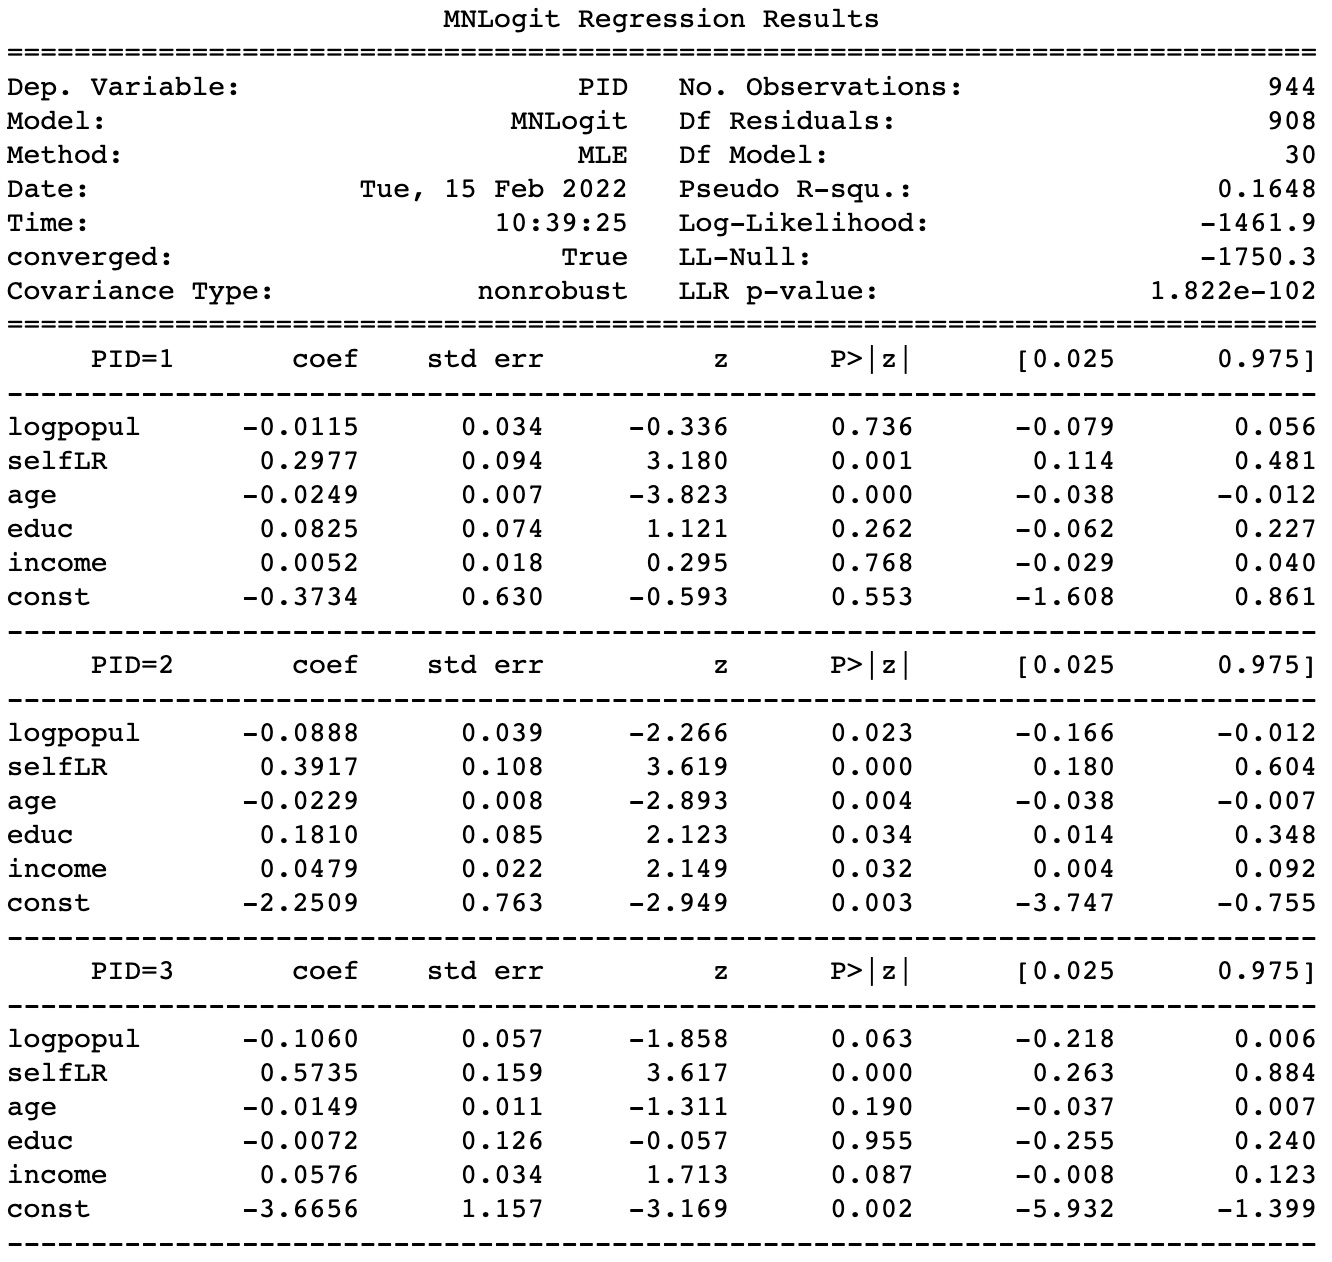
\includegraphics[scale=0.33]{./images/7.jpg}
\end{figure}
\begin{figure}[h!]
  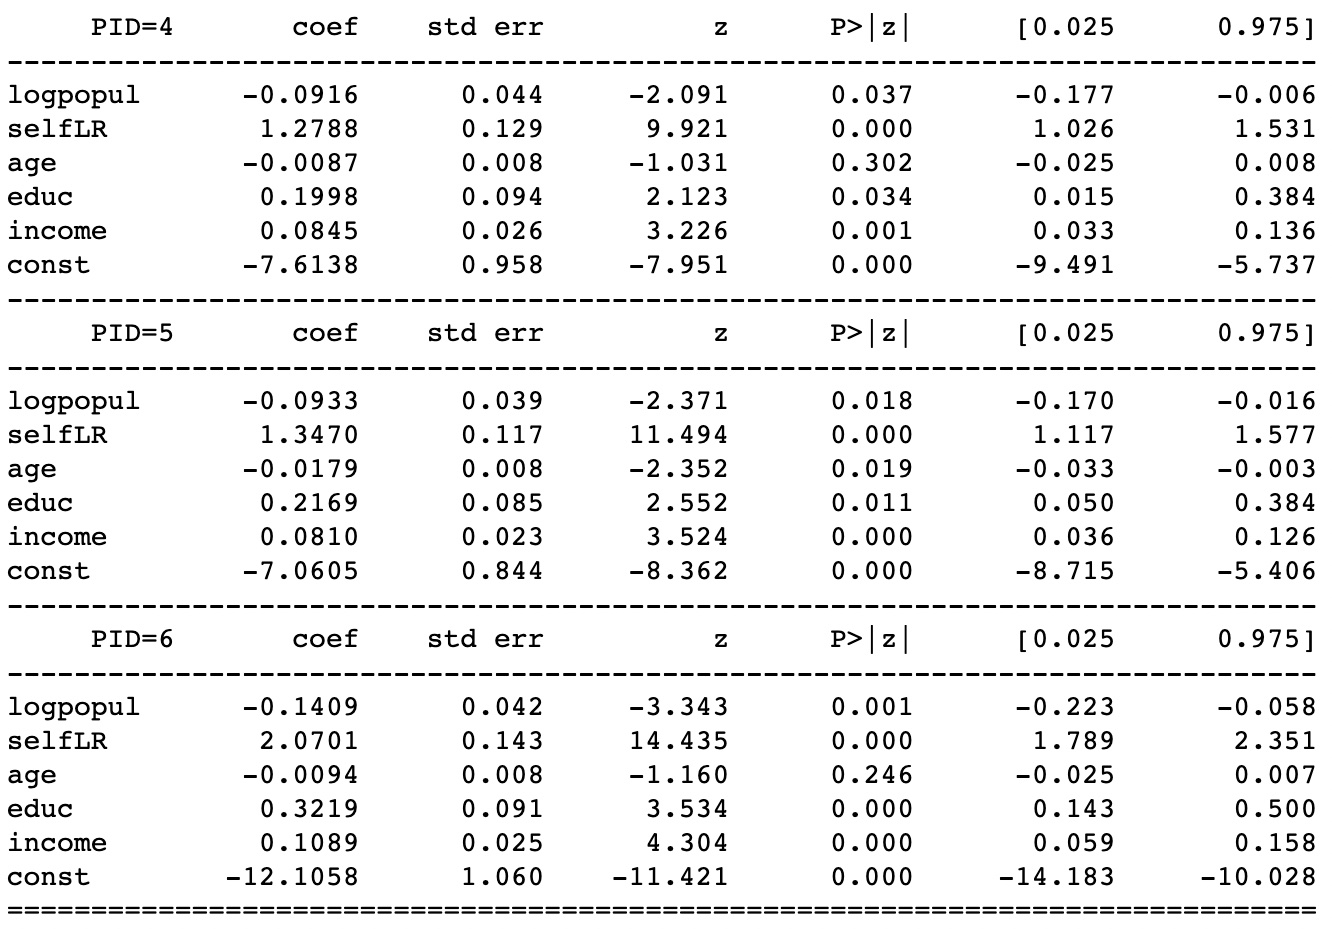
\includegraphics[scale=0.33]{./images/7_2.jpg}
\end{figure}
\clearpage
\subsection*{a)} This is because we are keeping a variable fixed, but at different values, which gives different coefficients.

\subsection*{b)} No, there are no features that are insignificant across the board.

\subsection*{c)} age is only significant for PID = 1, PID = 2, and PID = 5.

\subsection*{d)} selfLR is significant for all the classes. logpopul, const, educ, income are significant for most the classes.

\newpage
\section{Support Vector Machine}
\subsection*{a)} Plot shown below
\FloatBarrier
\begin{figure}[h!]
  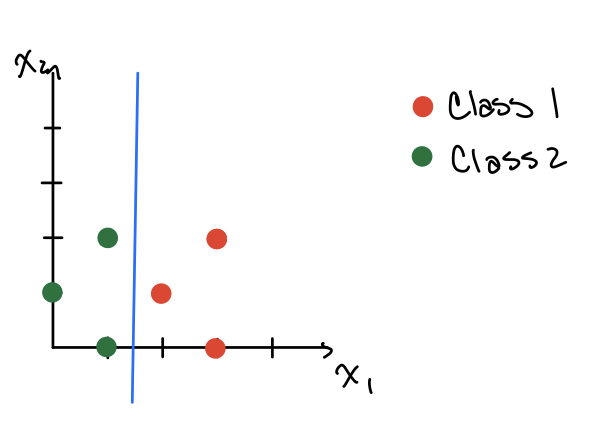
\includegraphics[scale=0.33]{./images/8a.jpg}
\end{figure}

\subsection*{b)} Points (1, 0), (1, 1), and (2, 1) are support vectors. If (2, 1) was removed, then the boundary would change.

\subsection*{c)} A hard margin is used for linearly separable data, and does not allow for misclassifcations. It tries to maxmimize the distance between data points and the boundary. Soft margin allows misclassification in hopes of achieving better generality, so it tries to minimize misclassification error. For this dataset, it doesn't matter whether use hard or soft margin, as they result in the same decision boundary.

\subsection*{d)} The left sub-figure corresponds to SVM (linear), because the decision boundary is linear. The middle sub-figure corresponds to SVM with polynomial kernel, because the decision boundary follows a polynomial curve. Finally, the right sub-figure corresponds to SVM with RBF kernel with width ($\gamma$) equal to 1, because the RBF kernel because it has a radius around each of the classes.
\begin{figure}[h!]
  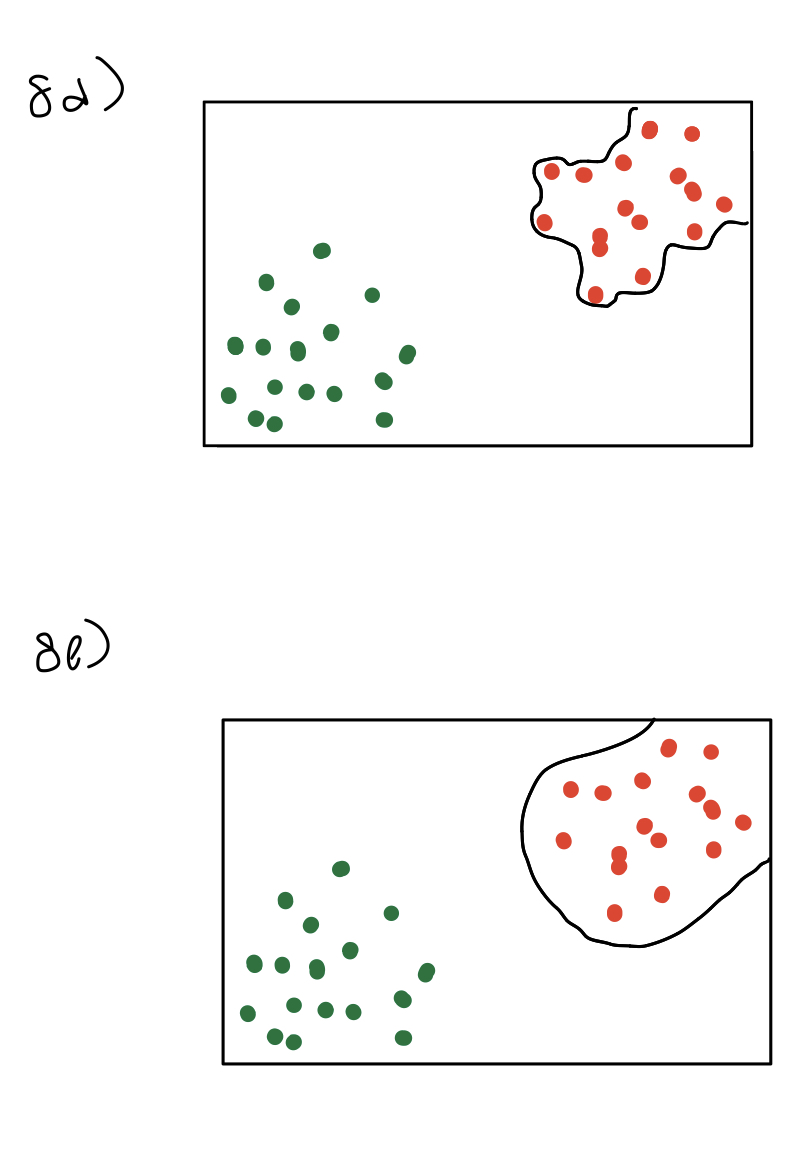
\includegraphics[scale=0.33]{./images/8ef.jpeg}
\end{figure}
\clearpage

\end{document}